\setcounter{chapter}{10}  % sets the current chapter to 10 so that the next one becomes 11

\chapter{Introduction to Hypothesis Testing}
\label{ch:intro-hypothesis}

\section{Test of Hypothesis for One Mean}

\begin{definition}[Hypothesis Tests]
An inferential procedure to determine whether there is sufficient evidence to suggest a condition for a population parameter using statistics from a sample.
\end{definition}


\textcolor{blue}{Attach a probability to the conclusion of a hypothesis test.}

\subsubsection*{Steps}
\begin{enumerate}
    \item Decide on a level of significance ($\alpha$)
    \item State the null hypothesis ($H_0$) and the alternative hypothesis ($H_a$) \textcolor{blue}{($H_1$)}
    \item Calculate the appropriate test statistic.
    \item Use the test statistic and a reference distribution to calculate a p-value. \\
    \textcolor{blue}{(Also refer back to $H_a$)}
    \item Compare p-value to $\alpha$ to make a conclusion.
\end{enumerate}

\textcolor{blue}{Note:} \\
\textcolor{blue}{The definition of a p-value can be confusing. We will define it later.}

\subsection*{Step 1: Decide on a Level of Significance ($\alpha$)}
-Threshold for decision making.

-Depends on tolerance for consequences of errors, sample size, nature of the study, and variability.

-Common values: $0.10$, $0.01$, $0.05$ \textcolor{blue}{(very common default)}

\subsection*{Step 2: State the Null Hypothesis ($H_0$) and the Alternative Hypothesis ($H_a$)}

\textbf{$\Theta$:} parameter of interest

\textbf{$\Theta_0$:} numerical value of the parameter of interest hypothesized under the null hypothesis.

\[
\begin{array}{lll}
H_0: \Theta = \Theta_0 & (\Theta \leq \Theta_0) & H_a: \Theta > \Theta_0 \quad \textcolor{blue}{\text{one-sided (one-tailed)}} \\
H_0: \Theta = \Theta_0 & (\Theta \geq \Theta_0) & H_a: \Theta < \Theta_0 \quad \textcolor{blue}{\text{one-sided (one-tailed)}} \\
H_0: \Theta = \Theta_0 &                         & H_a: \Theta \neq \Theta_0 \quad \textcolor{purple}{\text{two-sided (two-tailed)}}
\end{array}
\]


\textbf{Null ($H_0$):} Represents the current belief (\textcolor{blue}{status quo}) or the safe belief.

\textbf{Alternative ($H_a$):} Represents the research hypothesis (or what you are asked to test)
\subsection*{Step 3: Calculate an appropriate test statistic}

Depends on the hypothesis test conducted and the information available.


\begin{definition}[Test Statistic Skeleton]
\[
\text{test statistic} = \frac{\text{(a statistic)} - \text{(hypothesized value of parameters under } H_0 \text{)}}{\text{standard error of statistic}}
\]
\end{definition}

The test statistic follows a reference distribution ($Z$, $t$, $F$, $\chi^2$).
\subsection*{Step 4: Calculate the p-value}

\noindent
Use the test statistic, reference distribution, and refer back to $H_a$.

% --- BLUE: Right-tailed tests ---
\begin{figure}[H]
  \centering
  \begin{minipage}[t]{0.48\textwidth}
    \centering
    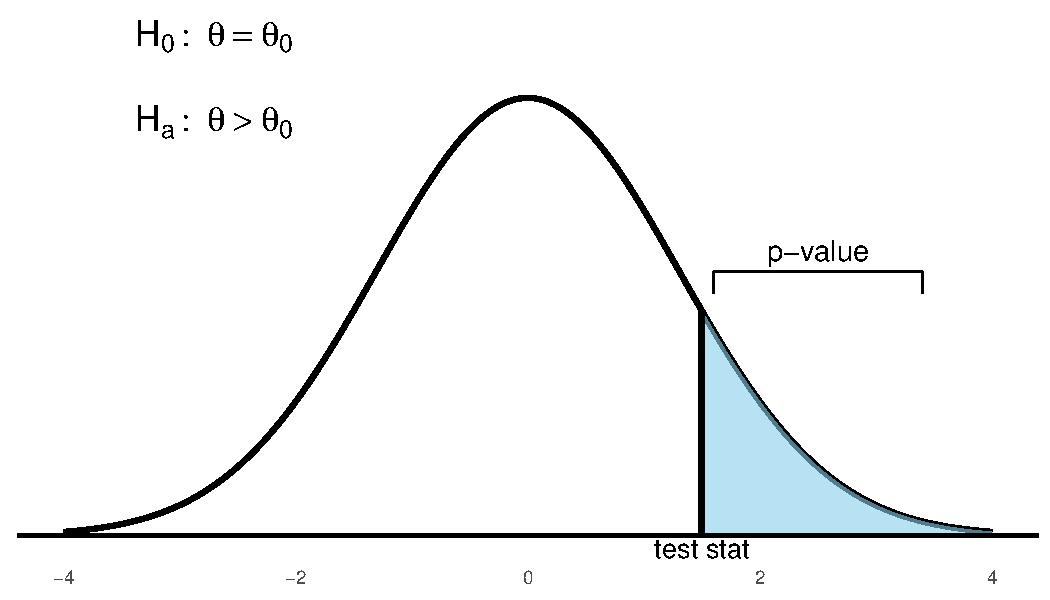
\includegraphics[width=\linewidth]{section11/images/hypothesis_right_tail.pdf}
  \end{minipage}
  \hfill
  \begin{minipage}[t]{0.48\textwidth}
    \centering
    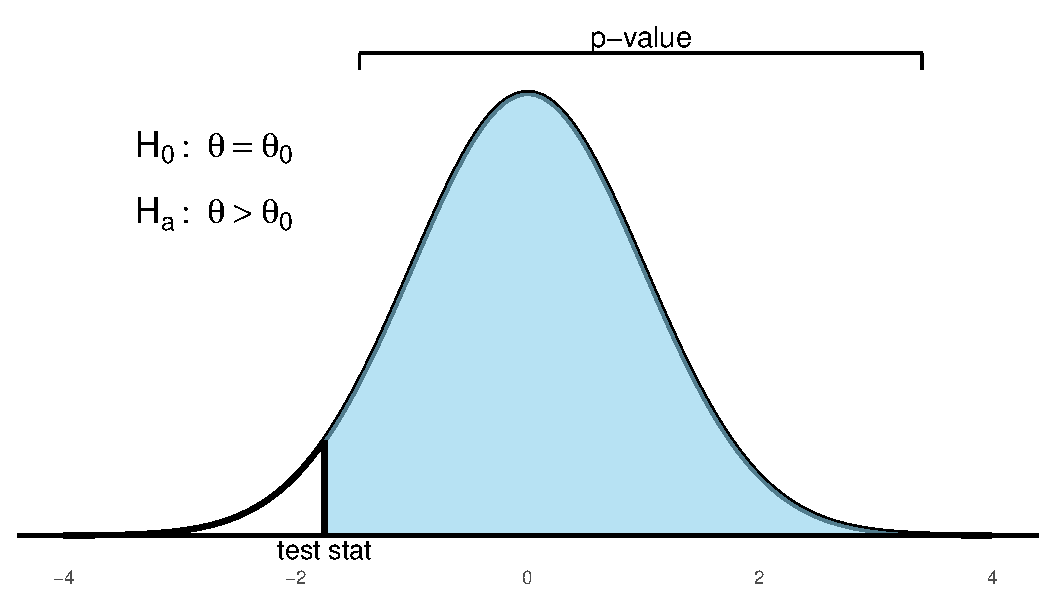
\includegraphics[width=\linewidth]{section11/images/hypothesis_right_tail_wide.pdf}
  \end{minipage}
  \caption{Right-tailed test: \textit{p}-value is the area to the right of the test statistic.}
\end{figure}


% --- PINK: Left-tailed tests ---
\begin{figure}[H]
  \centering
  \begin{minipage}{0.48\textwidth}
    \centering
    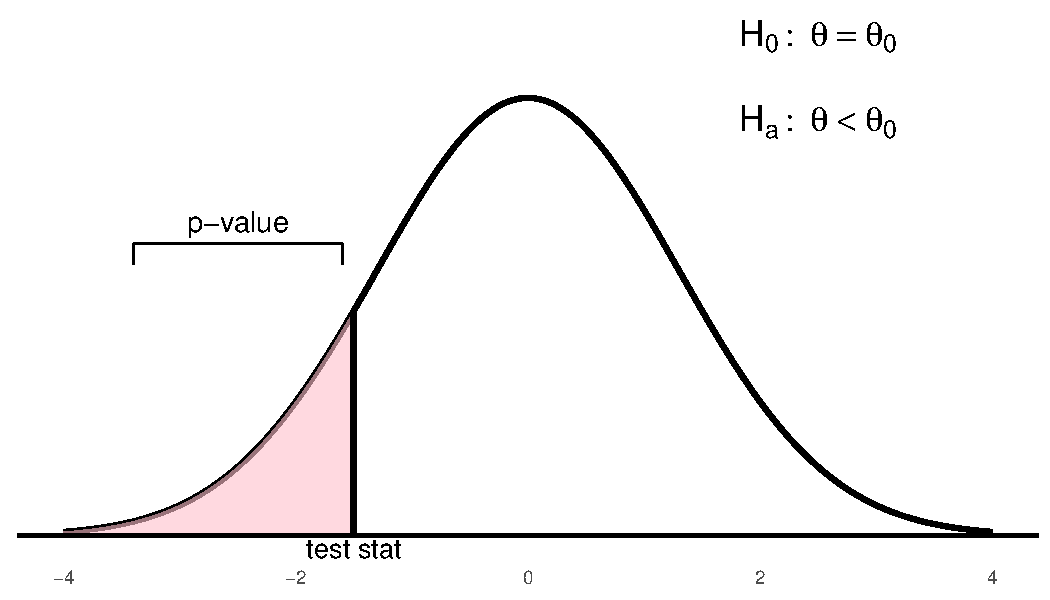
\includegraphics[width=\textwidth]{section11/images/hypothesis_left_tail.pdf}
  \end{minipage}
  \hfill
  \begin{minipage}{0.48\textwidth}
    \centering
    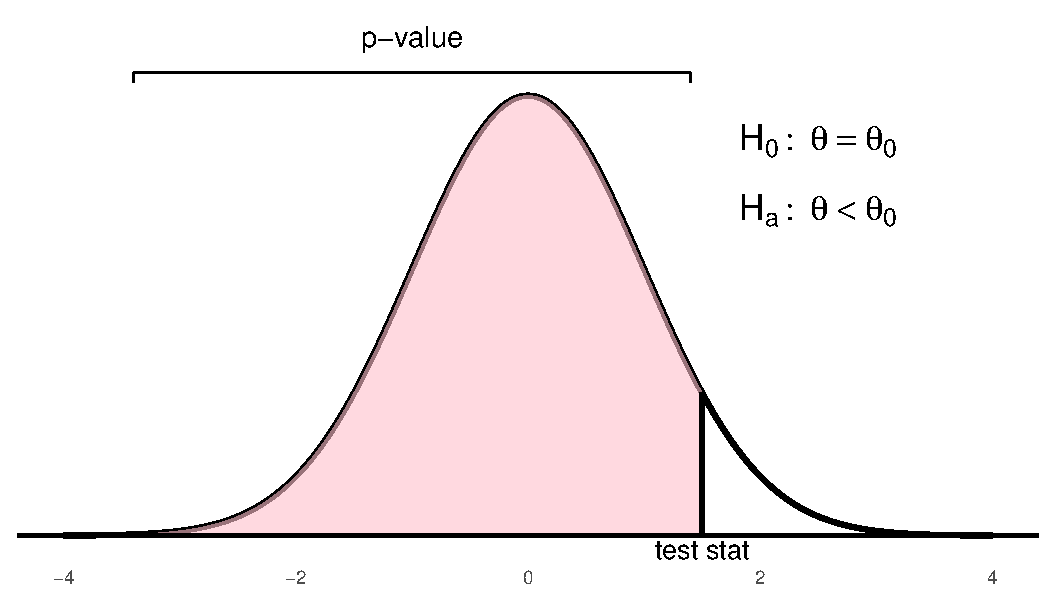
\includegraphics[width=\textwidth]{section11/images/hypothesis_left_tail_wide.pdf}
  \end{minipage}
\caption{Left-tailed test: \textit{p}-value is the area to the left of the test statistic.}
\end{figure}

% --- GREEN: Two-tailed test ---
\begin{figure}[H]
  \centering
  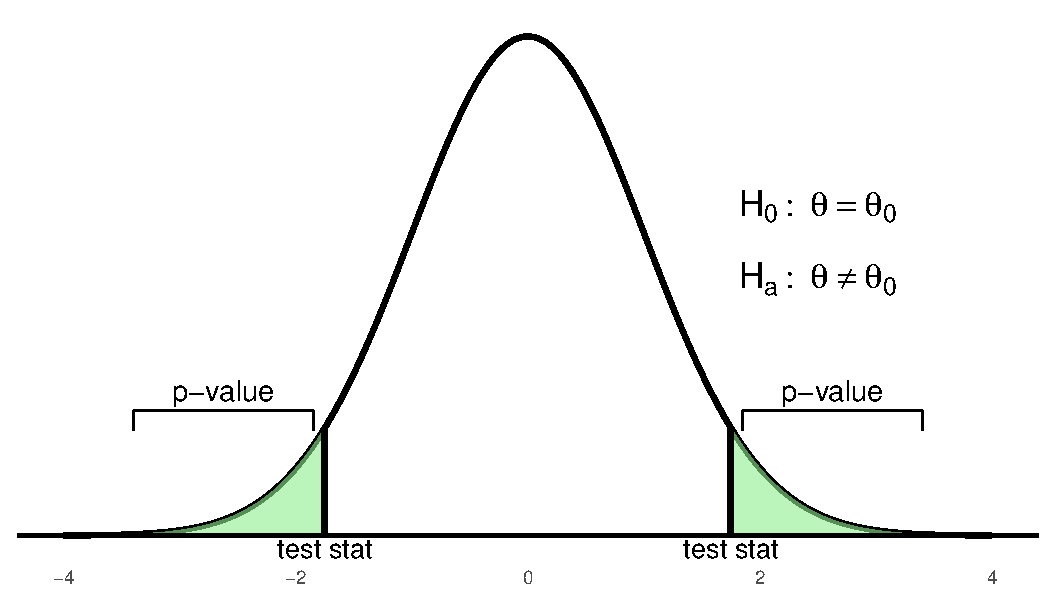
\includegraphics[width=0.52\textwidth]{section11/images/hypothesis_two_tail.pdf}
  \caption{Two-tailed test: p-value is the total area in both tails beyond $\pm$ test statistic.}
\end{figure}
\subsection*{Step 5: Compare \textit{p}-value to level of significance $\alpha$ and make a conclusion}

\begin{itemize}
  \item If \textit{p}-value $< \alpha$: \\
  \quad Sufficient evidence against $H_0$. The hypothesis test rejects $H_0$ in favor of $H_a$.

  \item If \textit{p}-value $> \alpha$: \\
  \quad Insufficient evidence against $H_0$. Do not reject $H_0$ (fail to reject $H_0$).
\end{itemize}

\textbf{Note:} It is not good practice to give conclusions in the context of stating we \textit{accept $H_0$} or \textit{accept $H_a$}.
\begin{example}[Sweetening Colas]
Diet colas use artificial sweeteners to avoid sugar. These sweeteners gradually lose their sweetness over time. Manufacturers therefore test new colas for loss of sweetness before marketing them. Trained tasters sip the cola along with drinks of standard sweetness and score the cola on a “sweetness score” of 1 to 10. The cola is then stored for a month at high temperature to imitate the effect of four months’ storage at room temperature. Each taster scores the cola again after storage. This is a matched pairs experiment. Our data are the differences (score before storage minus score after storage) in the tasters’ scores. The bigger these differences, the bigger the loss of sweetness.

Suppose we know that for any cola, the sweetness loss scores vary from taster to taster according to a Normal distribution with standard deviation $\sigma = 1$. The mean $\mu$ for all tasters measures loss of sweetness.

The following are the sweetness losses for a new cola as measured by 10 trained tasters:

\medskip
\centerline{2.0,\ 0.4,\ 0.7,\ 2.0,\ -0.4,\ 2.2,\ -1.3,\ 1.2,\ 1.1,\ 2.3}
\medskip

Are these data good evidence that the cola lost sweetness in storage?\\
\noindent\textbf{Solution}\\

$\mu$ = mean sweetness loss for the population of \textbf{all} tasters.\\
\textbf{Step 1:} State hypotheses.
\begin{align*}
H_0 &: \mu = 0 \\
H_a &: \mu > 0
\end{align*}
\textbf{Step 2:} Test statistic: $z_\star = \dfrac{\bar{x} - \mu_0}{\sigma / \sqrt{n}} = \dfrac{1.02 - 0}{1 / \sqrt{10}} = 3.23$ \\
\textbf{Step 3:} P-value. $P(Z > z_\star) = P(Z > 3.23) = 0.0006$ \\
\textbf{Step 4:} Conclusion. We would rarely observe a mean as large as 1.02 if $H_0$ were true. The small p-value provides strong evidence against $H_0$, supporting $H_a: \mu > 0$. That is, the mean sweetness loss is likely positive.

\vspace{1em}
\noindent\textbf{R code (Simulation)}

\begin{tcolorbox}[colback=gray!10, colframe=black!45, arc=2mm]
\begin{verbatim}
# n = sample size;
n<-10;
mu.zero<-0;
sigma<-1;
sigma.xbar<-sigma/sqrt(n);

# x bar = sample mean with 10 obs;
x.bar<-rnorm(1,mean=mu.zero,sd=sigma.xbar);
x.bar;

## [1] 0.3265859

# z.star = test statistic;
z.star<-(x.bar-mu.zero)/sigma.xbar;
z.star;

## [1] 1.032755
\end{verbatim}
\end{tcolorbox}
\vspace{1em}
\noindent\textbf{R code (10,000 Simulations)}

\begin{tcolorbox}[colback=gray!10, colframe=black!45, arc=2mm]
\begin{verbatim}
n <- 10;
mu.zero <- 0;
sigma <- 1;
sigma.xbar <- sigma / sqrt(n);
# x bar = sample mean with 10 obs;
# m = number of simulations;
m <- 10000;
x.bar <- rnorm(m, mean = mu.zero, sd = sigma.xbar);

# z.star = test statistic;
z.star <- (x.bar - mu.zero) / sigma.xbar;
hist(z.star, xlab = "differences", col = "blue");
\end{verbatim}
\end{tcolorbox}
\vspace{1em}
\noindent\textbf{Histogram from simulation (see Section 7 for R code format)}

\begin{figure}[H]
  \centering
  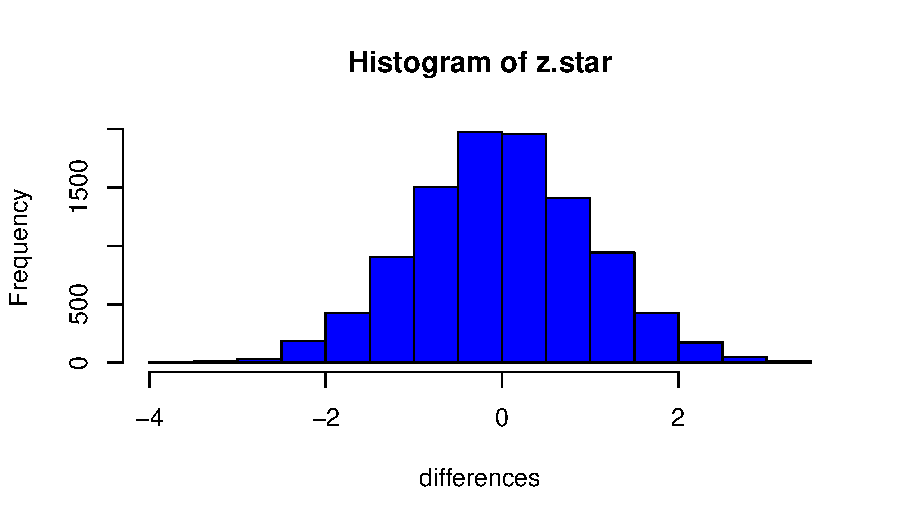
\includegraphics[width=0.6\textwidth]{Section11/images/sweetening_10000_hist.pdf}
  \vspace{-1em} % ← reduce space between figure and caption
\captionsetup{skip=0pt}
  \caption{Histogram of $z_\star$ values from 10,000 simulations under $H_0$.}
\end{figure}
\vspace{1em}
\noindent\textbf{R code (Empirical p-value)}

\begin{tcolorbox}[colback=gray!10, colframe=black!45, arc=2mm]
\begin{verbatim}
## P-value

p_value <- length(z.star[z.star > 3.23]) / m;

p_value

## [1] 8e-04
\end{verbatim}
\end{tcolorbox}


\end{example}
\begin{tcolorbox}[colback=yellow!5, colframe=yellow!50!black, title={One-Sample Hypothesis Test for Population Mean ($\mu$) (known  $\sigma$)}, sharp corners, boxrule=0.4pt, width=\textwidth, breakable]
\textbf{When $\sigma$ is known:}

\begin{tabular}{@{}ll@{\hspace{1.2cm}}ll@{}}
$\bullet\ H_0\!: \mu = \mu_0$ & (or $\mu \leq \mu_0$) & $H_a\!: \mu > \mu_0$ \\
$\bullet\ H_0\!: \mu = \mu_0$ & (or $\mu \geq \mu_0$) & $H_a\!: \mu < \mu_0$ \\
$\bullet\ H_0\!: \mu = \mu_0$ & & $H_a\!: \mu \neq \mu_0$ \\
\end{tabular}

\vspace{0.75em}
\begin{tabular}{@{}l l@{}}
\textbf{Test statistic:} & $z^* = \dfrac{\bar{X} - \mu_0}{\sigma/\sqrt{n}}$
\end{tabular}


\vspace{0.75em}
\textbf{Reference distribution:} Standard normal ($Z$)
\end{tcolorbox}
\begin{example}[UTM Deer]
Deer are a common sight on the UTM campus. Suppose an ecologist is interested in the average mass of adult white-tailed does (female deer) around the Mississauga campus to determine whether they are healthy for the upcoming winter. The ecologist captures a sample of 36 adult females around the UTM and measures the average mass of this sample to be 42.53 kg.

From previous studies conducted in the area, the average mass of healthy does was reported to be 45 kg. Conduct a hypothesis test at the 5\% significance level to determine whether the mass of does around UTM has decreased. Assume the standard deviation is known to be 5.25 kg.


\vspace{1em}

\textbf{1. Level of significance.} \(\alpha = 0.05\)

\textbf{2. State the null and alternative hypotheses.}
\[
H_0: \mu = 45 \qquad H_a: \mu < 45
\]

\textbf{3. Calculate appropriate test statistic.}

\vspace{0.5em}

Given:
\[
n = 36, \quad \bar{x} = 42.53, \quad \sigma = 5.25
\]

Since \(\sigma\) is known, the test statistic is:
\[
z^* = \frac{\bar{x} - \mu_0}{\sigma / \sqrt{n}} = \frac{42.53 - 45}{5.25/\sqrt{36}} = -2.82
\]

Reference distribution: standard normal

\textbf{4. Calculate p-value}

\[
\text{p-value} = P(Z < -2.82) \approx 0.0024
\]


\begin{figure}[H]
\centering
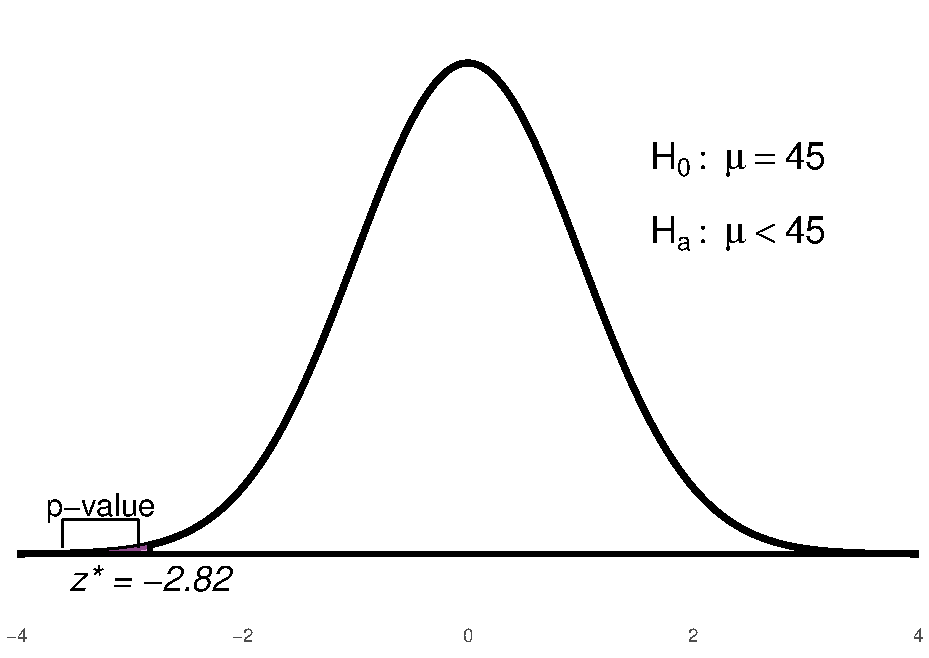
\includegraphics[width=0.6\textwidth]{section11/images/deer_pvalue.pdf}
\vspace{-0.25em} % ← reduce space between figure and caption
\captionsetup{skip=0pt}
\caption{Left-tailed p-value for the test statistic \( z^* = -2.82 \)}
\end{figure}

\textbf{5. Compare p-value with level of significance \(\alpha\) and make a conclusion:}

\[
0.0024 < 0.05 \Rightarrow \text{p-value} < \alpha
\]

There is sufficient evidence at the 5\% level of significance to reject the null that does this winter weigh the same as in the past and to conclude the alternative that does this winter weigh less than 45 kg.

\vspace{1em} % optional, if there's space needed above the label
\noindent\textbf{R code:}
\vspace{0.8em}
\begin{tcolorbox}[
  colback=gray!10, 
  colframe=black!45, 
  arc=2mm, 
  breakable, 
  after skip=0pt,  % no space after box
  before skip=0.3pt, % 🟢 key to tighten gap before box
  boxsep=1pt, left=4pt, right=4pt, top=2pt, bottom=2pt % 🟢 shrink padding
]
\begin{verbatim}
# Find test stat
z_test_stat = (42.53 - 45) / (5.25 / sqrt(36))
z_test_stat
[1] -2.822857

# Find the p-value
# Since the alternative is Ha : mu < 45
p-value = pnorm(z_test_stat)
[1] 0.00237989
\end{verbatim}
\end{tcolorbox}
\noindent\textit{Note:} The \texttt{pnorm()} function in R, by default, returns the cumulative probability (area) to the left of the given value. \\
\par\vspace{0.8em}  % <-- This forces the vertical break and then adds space
\noindent\textbf{R code: Using BSDA package}
\vspace{0.3em}

\begin{tcolorbox}[colback=gray!10, colframe=black!45, arc=2mm,
  breakable, boxsep=1pt, left=4pt, right=4pt, top=2pt, bottom=2pt,
  before skip=0pt, after skip=1em]
\small
\begin{verbatim}
# Using the BSDA library. install BSDA if it is not already installed.
# install.packages("BSDA")
> library(BSDA)
> # Conduct the z-test with the zsum.test function
> zsum.test(mean.x = 42.53, sigma.x = 5.24, n.x = 36, mu = 45, alternative = "less")

        One-sample z-Test

data:  Summarized x
z = -2.8282, p-value = 0.00234
alternative hypothesis: true mean is less than 45
95 percent confidence interval:
 NA 43.96651
sample estimates:
mean of x 
    42.53 
\end{verbatim}
\end{tcolorbox}

\vspace{1em}
\noindent\textbf{Interpretation:}

There is sufficient evidence at the 5\% level of significance to reject the null hypothesis. We conclude that the average mass of does this winter is significantly less than 45 kg.
\end{example}

\begin{example}[Executives’ Blood Pressures]

The National Center for Health Statistics reports that the systolic blood pressure for males 35 to 44 years of age has mean 128 and standard deviation 15. 

The medical director of a large company looks at the medical records of 72 executives in this age group and finds that the mean systolic blood pressure in this sample is $\bar{x} = 126.07$. Is this evidence that the company’s executives have a different mean blood pressure from the general population?

Suppose we know that executives’ blood pressures follow a Normal distribution with standard deviation $\sigma = 15$.

\textbf{Solution:} Let $\mu$ be the mean systolic blood pressure of the executive population.

\begin{enumerate}
    \item \textbf{State hypotheses:} \\
    \begin{align*}
H_0 &: \mu = 128 \\
H_a &: \mu \ne 128
\end{align*}

    
    \item \textbf{Test statistic:} \\
    \[
    z_\ast = \frac{\bar{x} - \mu_0}{\sigma / \sqrt{n}} = \frac{126.07 - 128}{15 / \sqrt{72}} = -1.09
    \]

    \item \textbf{P-value:} \\
    \[
    2P(Z > |z_\ast|) = 2P(Z > 1.09) = 2(1 - 0.8621) = 0.2758
    \]

    \item \textbf{Conclusion:} \\
    More than 27\% of the time, a simple random sample of size 72 from the general male population would have a mean blood pressure at least as far from 128 as that of the executive sample. The observed $\bar{x} = 126.07$ is therefore not good evidence that executives differ from other men.
\end{enumerate}

\end{example}
\begin{tcolorbox}[title=\textbf{Tests for a Population Mean},
  colback=yellow!10,
  colframe=black!45,
  coltitle=black,
  fonttitle=\bfseries,
  breakable]

There are four steps in carrying out a significance test:
\begin{enumerate}
  \item State the hypotheses.
  \item Calculate the test statistic.
  \item Find the P-value.
  \item State your conclusion in the context of your specific setting.
\end{enumerate}

Once you have stated your hypotheses and identified the proper test, you or your computer can do Steps 2 and 3 by following a recipe. 

\end{tcolorbox}
\begin{tcolorbox}[title=\textbf{Z Test for a Population Mean ($\mu$)},
  colback=yellow!10,
  colframe=black!45,
  coltitle=black,
  fonttitle=\bfseries,
  breakable]

Here is the recipe for the test we have used in our examples.\\
Draw a simple random sample of size $n$ from a Normal population that has unknown mean $\mu$ and known standard deviation $\sigma$.
To test the null hypothesis that $\mu$ has a specified value, $H_0 : \mu = \mu_0$, calculate the \textbf{one-sample $z$ statistic}:
\[
z_\ast = \frac{\bar{x} - \mu_0}{\sigma / \sqrt{n}}
\]

In terms of a variable $Z$ having the standard Normal distribution, the P-value for a test of $H_0$ against:
\begin{itemize}
  \item $H_a: \mu > \mu_0$ is $P(Z > z_\ast)$
  \item $H_a: \mu < \mu_0$ is $P(Z < z_\ast)$
  \item $H_a: \mu \ne \mu_0$ is $2P(Z > |z_\ast|)$
\end{itemize}

\end{tcolorbox}
\begin{example}

Consider the following hypothesis test:

\begin{align*}
H_0 &: \mu = 20 \\
H_a &: \mu < 20
\end{align*}


A sample of 50 provided a sample mean of 19.4. The population standard deviation is 2.

\begin{enumerate}
    \item[(a)] Compute the value of the test statistic.
    \item[(b)] What is the p-value?
    \item[(c)] Using $\alpha = 0.05$, what is your conclusion?
\end{enumerate}

\textbf{Solution:}

\begin{enumerate}
    \item[(a)] \textbf{Test statistic:}
    \[
    z_\ast = \frac{\bar{x} - \mu_0}{\sigma / \sqrt{n}} = \frac{19.4 - 20}{2 / \sqrt{50}} = -2.1213
    \]
    
    \item[(b)] \textbf{P-value:}
    \[
    P(Z < z_\ast) = P(Z < -2.1213) = 0.0169
    \]

    \item[(c)] \textbf{Conclusion:} \\
    Since the P-value $= 0.0169 < \alpha = 0.05$, we reject $H_0 : \mu = 20$. We conclude that $\mu < 20$.
\end{enumerate}

\end{example}
\begin{example}

Consider the following hypothesis test:

\begin{align*}
H_0 &: \mu = 25 \\
H_a &: \mu > 25
\end{align*}


A sample of 40 provided a sample mean of 26.4. The population standard deviation is 6.

\begin{enumerate}
    \item[(a)] Compute the value of the test statistic.
    \item[(b)] What is the p-value?
    \item[(c)] Using $\alpha = 0.01$, what is your conclusion?
\end{enumerate}

\textbf{Solution:}

\begin{enumerate}
    \item[(a)] \textbf{Test statistic:}
    \[
    z_\ast = \frac{\bar{x} - \mu_0}{\sigma / \sqrt{n}} = \frac{26.4 - 25}{6 / \sqrt{40}} = 1.4757
    \]

    \item[(b)] \textbf{P-value:}
    \[
    P(Z > z_\ast) = P(Z > 1.4757) = 0.0700
    \]

    \item[(c)] \textbf{Conclusion:} \\
    Since P-value $= 0.0700 > \alpha = 0.01$, we \textbf{cannot reject} $H_0 : \mu = 25$. \\
    We conclude that we don’t have enough evidence to claim that $\mu > 25$.
\end{enumerate}

\end{example}
\begin{example}

Consider the following hypothesis test:

\begin{align*}
H_0 &: \mu = 15 \\ 
H_a &: \mu \ne 15
\end{align*}

A sample of 50 provided a sample mean of 14.15. The population standard deviation is 3.

\begin{enumerate}
    \item[(a)] Compute the value of the test statistic.
    \item[(b)] What is the p-value?
    \item[(c)] Using $\alpha = 0.05$, what is your conclusion?
\end{enumerate}

\textbf{Solution:}

\begin{enumerate}
    \item[(a)] \textbf{Test statistic:}
    \[
    z_\ast = \frac{\bar{x} - \mu_0}{\sigma / \sqrt{n}} = \frac{14.15 - 15}{3 / \sqrt{50}} = -2.0034
    \]

    \item[(b)] \textbf{P-value:}
    \[
    2P(Z > |z_\ast|) = 2P(Z > |{-2.0034}|) = 2P(Z > 2.0034) = 0.0451
    \]

    \item[(c)] \textbf{Conclusion:} \\
    Since P-value $= 0.0451 < \alpha = 0.05$, we reject $H_0 : \mu = 15$. \\
    We conclude that $\mu \ne 15$.
\end{enumerate}

\textbf{Confidence Interval Interpretation:}

The 95\% confidence interval for $\mu$ is:
\[
\bar{x} \pm z_\ast \left( \frac{\sigma}{\sqrt{n}} \right)
\]
\[
14.15 \pm 1.96 \left( \frac{3}{\sqrt{50}} \right)
= (13.3184,\ 14.9815)
\]

Since the hypothesized value $\mu_0 = 15$ falls \textbf{outside} this interval, we again reject $H_0 : \mu = 15$.

\end{example}
\begin{nt}[Confidence Intervals and Two-Sided Tests]
\textit{
A level $\alpha$ two-sided significance test rejects a hypothesis $H_0 : \mu = \mu_0$ exactly when the value $\mu_0$ falls outside a level $1 - \alpha$ confidence interval for $\mu$.
}

\end{nt}
\begin{tcolorbox}[colback=yellow!5, colframe=yellow!50!black, 
  title={One-Sample Hypothesis Test for Population Mean ($\mu$) (unknown $\sigma$)},
  sharp corners, boxrule=0.4pt, width=\textwidth, breakable]
\textbf{When $\sigma$ is NOT known:}

\begin{tabular}{@{}ll@{\hspace{1.2cm}}ll@{}}
$\bullet$ H$_0\!$ : $\mu = \mu_0$ & (or $\mu \geq \mu_0$) & $H_a\!$ : $\mu < \mu_0$ \\
$\bullet$ H$_0\!$ : $\mu = \mu_0$ & (or $\mu \leq \mu_0$) & $H_a\!$ : $\mu > \mu_0$ \\
$\bullet$ H$_0\!$ : $\mu = \mu_0$ & & $H_a\!$ : $\mu \ne \mu_0$
\end{tabular}

\vspace{0.75em}
\begin{tabular}{@{}l @{}}
\textbf{Test statistic:} $t^\ast = \dfrac{\bar{X} - \mu_0}{s / \sqrt{n}}$
\end{tabular}

\vspace{0.75em}
\textbf{Reference distribution:} $t$ distribution with $n - 1$ degrees of freedom

\end{tcolorbox}
\begin{example}[Hypothesis Test: Laughter and Heart Rate, Unknown $\sigma$]

Researchers studied the physiological effects of laughter. They measured heart rates (in beats per minute) of \textbf{$n = 25$} subjects (ages 18–34) while they laughed. They obtained:
\[
\bar{x} = 73.5, \quad s = 6, \quad \alpha = 0.05
\]
It is well known that the resting heart rate is 71 bpm. Is there evidence that the mean heart rate during laughter exceeds 71 bpm?

\textbf{Step 1: State the hypotheses.}
\[
\begin{aligned}
H_0 &: \mu = 71 \\
H_a &: \mu > 71
\end{aligned}
\]

\textbf{Step 2: Check assumptions.}
\begin{itemize}
  \item The sample is an independent random sample of individuals aged 18–34.
  \item The population of heart rates during laughter is normally distributed.
\end{itemize}

\textbf{Step 3: Compute the test statistic.}

Since $\sigma$ is unknown, we use the $t$ statistic:
\[
t^\ast = \frac{\bar{x} - \mu_0}{s / \sqrt{n}} = \frac{73.5 - 71}{6 / \sqrt{25}} = 2.083
\]

Reference distribution: $t$ distribution with $n - 1 = 25 - 1 = 24$ degrees of freedom.

\textbf{Step 4: Determine the p-value.}

Using the $t$ distribution with 24 df:
\[
0.01 < \text{p-value} < 0.025
\]

\textbf{Step 5: Make a conclusion.}

Since $\text{p-value} < \alpha = 0.05$, we reject $H_0$.

\textit{There is sufficient evidence at the 5\% level of significance to reject the null that the mean is 71 bpm in favor of the alternative that the mean is greater than 71 bpm for people who are laughing.}


\end{example}
\begin{example}

A researcher is asked to test the hypothesis that the average price of a 2-star (CAA rating) motel room has decreased since last year. Last year, a study showed that the prices were Normally distributed with a mean of \$89.50.

A random sample of twelve 2-star motels produced the following room prices:

\[
\text{\$85.00, 92.50, 87.50, 89.90, 90.00, 82.50, 87.50, 90.00, 85.00, 89.00, 91.50, 87.50}
\]

At the 5\% level of significance, can we conclude that the mean price has decreased?

\textbf{Solution:}

Let $\mu$ be the true average price of a 2-star motel room.

\begin{enumerate}
  \item \textbf{State hypotheses.}
\begin{align*}
H_0 &: \mu = 89.5 \\
H_a &: \mu < 89.5
\end{align*}


  \item \textbf{Compute test statistic.}
  \[
  t^\ast = \frac{\bar{x} - \mu_0}{s / \sqrt{n}} = \frac{88.1583 - 89.5}{2.9203 / \sqrt{12}} = -1.5915
  \]

  \item \textbf{Find the P-value.} \\
  With $df = 11$, the P-value (from the $t$-distribution table) is between 0.05 and 0.10.

  \item \textbf{Conclusion.} \\
  Since P-value $> 0.05$, we \textbf{fail to reject} $H_0$. \\
  There is not sufficient evidence to conclude that the average price of 2-star motels has decreased this year.
\end{enumerate}
\vspace{1em}
\noindent\textbf{R code (One Sample t-test)}
\begin{tcolorbox}[colback=gray!10, colframe=black!45, arc=2mm]
\begin{verbatim}
# Step 1. Entering data;
prices=c(85.00, 92.50, 87.50, 89.90, 90.00, 82.50,
         87.50, 90.00, 85.00, 89.00, 91.50, 87.50);

# Step 2. Hypothesis test;
t.test(prices, alternative="less", mu=89.5);
\end{verbatim}
\end{tcolorbox}
\vspace{1em}
\noindent\textbf{R output}
\begin{tcolorbox}[colback=gray!10, colframe=black!45, arc=2mm]
\begin{verbatim}
## 
##  One Sample t-test
## 
## data:  prices
## t = -1.5915, df = 11, p-value = 0.0699
## alternative hypothesis: true mean is less than 89.5
## 95 percent confidence interval:
##  -Inf 89.67229
## sample estimates:
## mean of x 
##  88.15833 
\end{verbatim}
\end{tcolorbox}


\end{example}

\begin{tcolorbox}[title=\textbf{The one-sample \textit{t} test},
  colback=yellow!10,
  colframe=black!45,
  coltitle=black,
  fonttitle=\bfseries,
  breakable]

Draw an SRS of size $n$ from a large population having unknown mean $\mu$.

To \textit{test the hypothesis} $H_0 : \mu = \mu_0$, compute the \textit{one-sample $t$ statistic}
\[
t^\ast = \frac{\bar{x} - \mu_0}{s / \sqrt{n}}
\]

In terms of a variable $T$ having the $t_{n - 1}$ distribution, the P-value for a test of $H_0$ against

\begin{align*}
H_a : \mu > \mu_0 &\quad \text{is} \quad P(T \ge t^\ast) \\
H_a : \mu < \mu_0 &\quad \text{is} \quad P(T \le t^\ast) \\
H_a : \mu \ne \mu_0 &\quad \text{is} \quad 2P(T \ge |t^\ast|)
\end{align*}

These P-values are exact if the population distribution is Normal and are approximately correct for large $n$ in other cases.

\end{tcolorbox}
\begin{example}
We are conducting a two-sided one-sample $t$-test for the hypotheses:
\begin{align*}
H_0 &: \mu = 64 \\
H_a &: \mu \ne 64
\end{align*}

based on a sample of $n = 15$ observations, with test statistic $t^* = 2.12$.

\textbf{a) Degrees of freedom:}

\[
df = n - 1 = 15 - 1 = 14
\]

\textbf{b) Critical values and P-value bounds:}

From the $t$-distribution table for $df = 14$:

\begin{itemize}
  \item $t = 1.761$ corresponds to a two-tailed probability of 0.10
  \item $t = 2.145$ corresponds to a two-tailed probability of 0.05
\end{itemize}

Since $t^* = 2.12$ falls between these values, the two-sided P-value satisfies:
\[
0.05 < \text{P-value} < 0.10
\]

\textbf{c) Significance:}

\begin{itemize}
  \item At the 10\% level: \textbf{Yes}, since P-value $< 0.10$
  \item At the 5\% level: \textbf{No}, since P-value $> 0.05$
\end{itemize}

\textbf{d) Exact two-sided P-value using R:}

\begin{tcolorbox}[colback=gray!10, colframe=black!45, arc=2mm]
\begin{verbatim}
# Compute exact two-sided P-value for t* = 2.12 with df = 14
2 * (1 - pt(2.12, df = 14))

## [1] 0.05235683
\end{verbatim}
\end{tcolorbox}

Thus, the exact two-sided P-value is approximately \textbf{0.0524}, confirming the bracketing result.
\end{example}

\section{Test of Hypothesis for One Proportion}
\begin{tcolorbox}[colback=yellow!5, colframe=yellow!50!black, title={One-Sample Hypothesis Test for Population Proportion ($p$)}, sharp corners, boxrule=0.4pt, width=\textwidth, breakable]
\textbf{When sample size is large enough (np, n(1-p) $\ge$ 10):}

\begin{tabular}{@{}ll@{\hspace{1.2cm}}ll@{}}
$\bullet$ $H_0\!$ : $p = p_0$ & (or $p \geq p_0$) & $H_a\!$ : $p < p_0$ \\
$\bullet$ $H_0\!$ : $p = p_0$ & (or $p \leq p_0$) & $H_a\!$ : $p > p_0$ \\
$\bullet$ $H_0\!$ : $p = p_0$ & & $H_a\!$ : $p \ne p_0$
\end{tabular}



\vspace{0.75em}
\begin{tabular}{@{}l@{}}
\textbf{Test statistic:} $z^* = \dfrac{\hat{p} - p_0}{\sqrt{\dfrac{p_0(1 - p_0)}{n}}}$
\end{tabular}

\vspace{0.75em}
\textbf{Reference distribution:} Standard normal ($\mathcal{Z}$)
\end{tcolorbox}
\begin{example}[100-Cup Challenge]
A YouTuber goes to her nearest Tim Hortons and buys 100 empty cups. After rolling up the rims, she ends up with 12 winning cups out of the 100 she bought, all of them were food prizes.

If the probability of winning a food prize is supposed to be $\frac{1}{6}$, does she have evidence to claim that the probability of winning a food prize is less than $\frac{1}{6}$?
\end{example}
\begin{definition}
The \textbf{sample space} $\mathbf{S}$ of a random phenomenon is the set of all possible outcomes.

An \textbf{event} is an outcome or a set of outcomes of a random phenomenon. That is, an event is a subset of the sample space.

A \textbf{probability model} is a mathematical description of a random phenomenon consisting of two parts: a sample space $S$ and a way of assigning probabilities to events.
\end{definition}

Rolling a fair die (random phenomenon). There are 6 possible outcomes when we roll a die.\\
The sample space for rolling a die and counting the pips is

\[
S = \{1,\, 2,\, 3,\, 4,\, 5,\, 6\}
\]

“Roll a 6” is an event that contains one of these 6 outcomes.
\begin{definition}
A random variable $X$ has a \textbf{discrete uniform distribution} if each of the $n$ values in its range, say, $x_1, x_2, \ldots, x_n$, has equal probability. Then,
\[
f(x_i) = \frac{1}{n}
\]
\end{definition}
\vspace{1em}
\noindent\textbf{R code: }

\begin{tcolorbox}[colback=gray!10, colframe=black!45, arc=2mm]
\begin{verbatim}
# Define a die with values 1 through 6
die <- c(1, 2, 3, 4, 5, 6)

# Roll the die once
sample(die, 1, replace = TRUE)
## [1] 2

# Roll the die six times
sample(die, 6, replace = TRUE)
## [1] 1 3 2 6 3 1
\end{verbatim}
\end{tcolorbox}
\vspace{1em}

\begin{figure}[H]
  \centering
  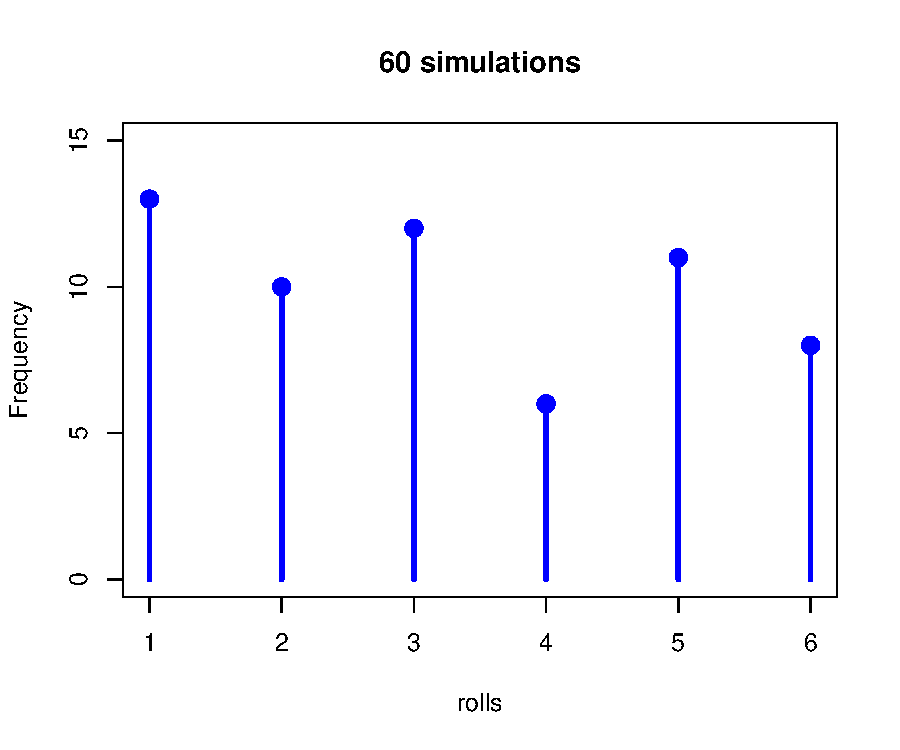
\includegraphics[width=0.6\textwidth]{section11/images/simulation_60.pdf} 
  \vspace{-1em} % ← reduce space between figure and caption
\captionsetup{skip=0pt}
  \caption{Plot of frequencies from 60 simulations of a fair six-sided die.}
\end{figure}
\begin{definition}
A \textbf{random variable} is a variable whose value is a numerical outcome of a random phenomenon.

The \textbf{probability distribution} of a random variable $X$ tells us what values $X$ can take and how to assign probabilities to those values.
\end{definition}
\begin{nt}{The Binomial setting}
\begin{itemize}
  \item There are a fixed number $n$ of observations.
  \item The $n$ observations are all \textbf{independent}. That is, knowing the result of one observation tells you nothing about the other observations.
  \item Each observation falls into one of just two categories, which for convenience we call “success” and “failure”.
  \item The probability of a success, call it $p$, is the same for each observation.
\end{itemize}
\end{nt}
\noindent A random variable $Y$ is said to have a \textbf{binomial distribution} based on $n$ trials with success probability $p$ if and only if
\[
p(y) = \frac{n!}{y!(n - y)!} \, p^y (1 - p)^{n - y}, \quad y = 0, 1, 2, \ldots, n \quad \text{and} \quad 0 \leq p \leq 1.
\]
\begin{example}
Think of rolling a die $n$ times as an example of the binomial setting. Each roll gives either a six or a number different from six. Knowing the outcome of one roll doesn’t tell us anything about other rolls, so the $n$ rolls are independent. 

If we call six a success, then $p$ is the probability of a six and remains the same as long as we roll the same die. The number of sixes we count is a random variable $X$. The distribution of $X$ is called a \textbf{binomial distribution}.
\end{example}
\vspace{1em}
\noindent\textbf{R code (Binomial Simulations and PMF)}

\begin{tcolorbox}[colback=gray!10, colframe=black!45, arc=2mm]
\begin{verbatim}
## Simulation: Binomial with n = 10 and p = 1/6.
rbinom(1, size = 10, prob = 1/6);
## [1] 3

rbinom(1, size = 10, prob = 1/6);
## [1] 1

rbinom(1, size = 10, prob = 1/6);
## [1] 0

## Pmf: Binomial with n = 10 and p = 1/6.
x <- seq(0, 10, by = 1);
y <- dbinom(x, 10, 1/6);
plot(x, y, type = "p", col = "blue", pch = 19);
\end{verbatim}
\end{tcolorbox}
\vspace{1em}

\begin{figure}[H]
  \centering
  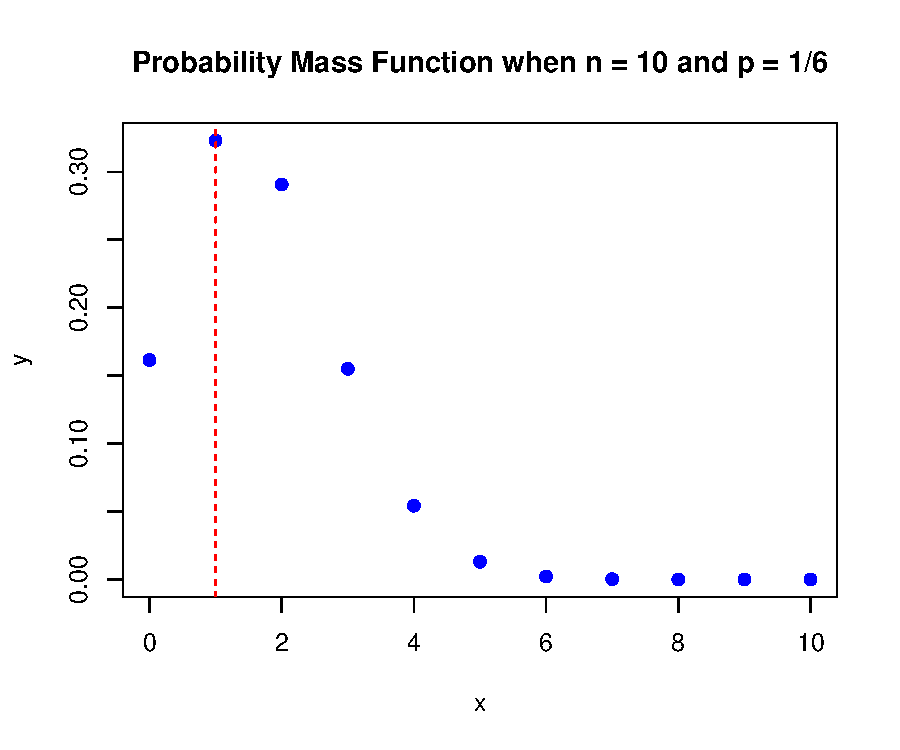
\includegraphics[width=0.65\textwidth]{section11/images/binomial_pmf.pdf}
  \vspace{-1em} % ← reduce space between figure and caption
\captionsetup{skip=0pt}
  \caption{PMF when $n=10$ and $p=1/6$}
\end{figure}

\vspace{1em}

\begin{figure}[H]
  \centering
  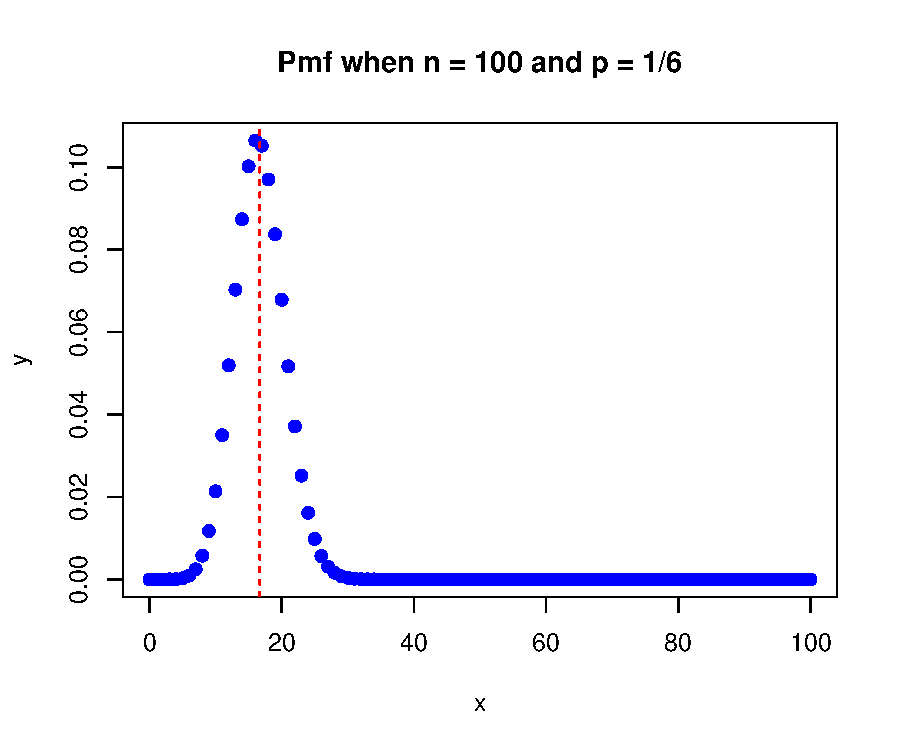
\includegraphics[width=0.65\textwidth]{section11/images/binomial_pmf_100.pdf}
  \vspace{-1em} % ← reduce space between figure and caption
\captionsetup{skip=0pt}
  \caption{PMF when $n=100$ and $p=1/6$}
\end{figure}
\vspace{1em}
\noindent\textbf{R code (PMF values for selected $x$ values)}

\begin{tcolorbox}[colback=gray!10, colframe=black!45, arc=2mm]
\begin{verbatim}
dbinom(c(15, 16, 17, 18), size = 100, prob = 1/6);
## [1] 0.10023663 0.10650142 0.10524847 0.09706247
\end{verbatim}
\end{tcolorbox}
\vspace{1em}
\begin{figure}[H]
  \centering
  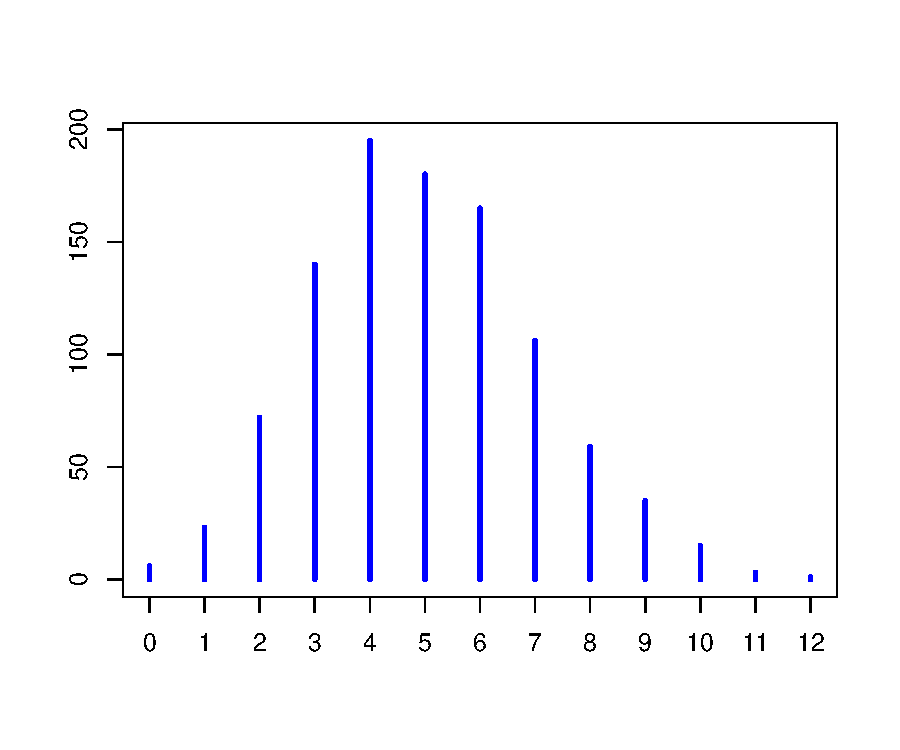
\includegraphics[width=0.65\textwidth]{section11/images/binomial_simulation_histogram.pdf}
  \vspace{-2em} % ← reduce space between figure and caption
\captionsetup{skip=0pt}
  \caption{Simulation: 2000 YouTuber, $n = 100$, and $p = 1/6$}
\end{figure}
\vspace{1em}
\noindent\textbf{R code (A few values from our simulation)}

\begin{tcolorbox}[colback=gray!10, colframe=black!45, arc=2mm]
\begin{verbatim}
## vec.prop
##  6  7  8  9 10 11 12 
##  7  3  8 24 46 72 106 
## [1] 266
## [1] 0.133
\end{verbatim}
\end{tcolorbox}
\vspace{1em}

It turns out that our P-value for this simulation is: \\
0.133
\begin{figure}[H]
  \centering
  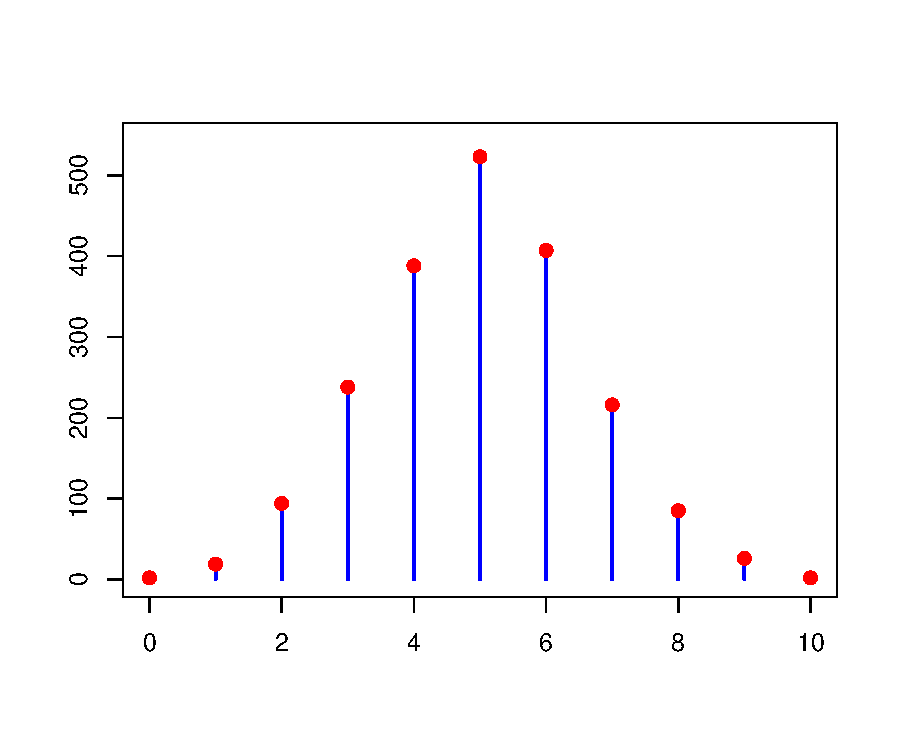
\includegraphics[width=0.65\textwidth]{section11/images/sim_vs_theoretical_pmf.pdf}
  \vspace{-2em} % ← reduce space between figure and caption
\captionsetup{skip=0pt}
  \caption{Simulation vs Theoretical pmf}
\end{figure}
\begin{tcolorbox}[colback=yellow!5, colframe=yellow!50!black, title={Sampling Distribution of a Sample Proportion}, sharp corners, boxrule=0.4pt, width=\textwidth, breakable]

Draw an SRS of size $n$ from a large population that contains proportion $p$ of “successes”. Let $\hat{p}$ be the \textbf{sample proportion} of successes,

\[
\hat{p} = \frac{\text{number of successes in the sample}}{n}
\]

Then:

\begin{itemize}
  \item The \textbf{mean} of the sampling distribution of $\hat{p}$ is $p$.
  \item The \textbf{standard deviation} of the sampling distribution is
  \[
  \sqrt{\frac{p(1 - p)}{n}}.
  \]
\end{itemize}

\vspace{0.75em}

\begin{itemize}
  \item As the sample size increases, the sampling distribution of $\hat{p}$ becomes \textbf{approximately Normal}. That is, for large $n$, $\hat{p}$ has approximately the
  \[
  N\left(p, \sqrt{\frac{p(1 - p)}{n}}\right)
  \]
  distribution.
\end{itemize}

\end{tcolorbox}
\begin{figure}[H]
  \centering
  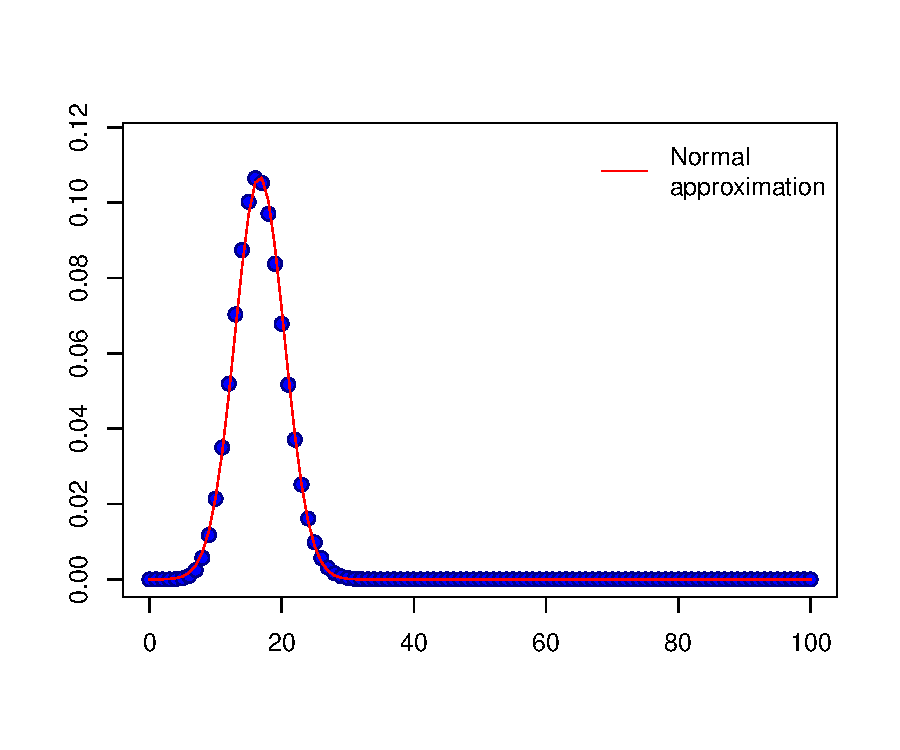
\includegraphics[width=0.65\textwidth]{section11/images/binomial_normal_approximation.pdf}
  \vspace{-2em} % ← reduce space between figure and caption
\captionsetup{skip=0pt}
  \caption{Binomial with Normal Approximation}
\end{figure}
\begin{tcolorbox}[title=\textbf{Hypotheses Tests for a Proportion},
colback=yellow!10,
colframe=black!45,
coltitle=black,
fonttitle=\bfseries,
breakable]

To \textit{test the hypothesis} $H_0 : p = p_0$, compute the $z_\ast$ statistic:
\[
z_\ast = \frac{\hat{p} - p_0}{\sqrt{\dfrac{p_0(1 - p_0)}{n}}}
\]

In terms of a variable $Z$ having the standard Normal distribution, the approximate P-value for a test of $H_0$ against:

\begin{align*}
H_a &: p > p_0 \quad \text{is} \quad P(Z > z_\ast) \\
H_a &: p < p_0 \quad \text{is} \quad P(Z < z_\ast) \\
H_a &: p \ne p_0 \quad \text{is} \quad 2P(Z > |z_\ast|) \\
\end{align*}

\end{tcolorbox}
\section*{Introduction to Hypothesis Testing (Significance Test)}

Consider the following problem: In 1980s, it was generally believed that congenital abnormalities affect 5\% of the nation’s children. Some people believe that the increase in the number of chemicals in the environment in recent years has led to an increase in the incidence of abnormalities. A recent study examined 384 children and found that 46 of them showed signs of abnormality. Is this strong evidence that the risk has increased?

\begin{itemize}
  \item The above statement serves as a hypothesis, moreover it is a Research Hypothesis.
\end{itemize}

A hypothesis is:

\begin{itemize}
  \item a statement about a population.
  \item a prediction that a parameter describing some characteristics of a variable (e.g., true proportion, $p$) takes a particular numerical value or falls in a certain range of values.
\end{itemize}

\vspace{1em}

For conducting a Significance Test:

\begin{itemize}
  \item Researchers (you) use data to summarize the evidence about a hypothesis.
  \item With data, you can compare the point estimates of parameters to the values predicted by the hypothesis.
\end{itemize}

\vspace{1em}

\textbf{Important Ideas about Hypothesis Testing}

\begin{itemize}
  \item All the hypothesis tests boil down to the same question: “Is an observed difference or pattern too large to be attributed to chance?”
  \item We measure “how large” by putting our sample results in the context of a sampling distribution model (e.g., Normal model, $t$ distribution).
\end{itemize}

\vspace{1em}

To plan a statistical hypothesis test, specify the model you will use to test the null hypothesis and the parameter of interest.

\begin{itemize}
  \item All models require assumptions, so you will need to state them and check any corresponding conditions.
  \item For example, if the conditions are satisfied, we can model the sampling distribution of the proportion with a Normal model. Otherwise, we cannot proceed with the test (we need to stop and reconsider).
\end{itemize}
\section*{Steps in conducting Hypothesis Testing}

\begin{enumerate}
  \item State the null and the alternative hypothesis.
  \item Check the necessary assumptions.
  \item Identify the test-statistic. Find the value of the test-statistic.
  \item Find the p-value of the test-statistic.
  \item State (if any) a conclusion.
\end{enumerate}

\begin{example}
\textbf{Example of Hypothesis Testing for a Proportion}

In 1980s, it was generally believed that congenital abnormalities affect 5\% of the nation’s children. Some people believe that the increase in the number of chemicals in the environment in recent years has led to an increase in the incidence of abnormalities. A recent study examined 384 children and found that 46 of them showed signs of abnormality. Is this strong evidence that the risk has increased?

\vspace{1em}
\textbf{Step 1. Set up the null and alternative hypothesis:}

\begin{itemize}
  \item The null hypothesis is the current belief: $H_0 : p = p_0$
\end{itemize}

In our example it would have a form: $H_0 : p = 0.05$

\begin{itemize}
  \item The Alternative hypothesis is what the researcher(s) [you] want to prove: $H_a : p > p_0$
\end{itemize}

In our example it would have a form: $H_a : p > 0.05$

This means a one-sided test.

\begin{itemize}
  \item The goal here is to provide evidence against $H_0$ (e.g., suggest $H_a$).
\end{itemize}

You want to conclude $H_a$. \\
Try a Proof by Contradiction: Assume $H_0$ is true \dots and hope your data contradicts it.

\vspace{1em}
\textbf{Step 2. Check the Necessary Assumptions:}

\begin{itemize}
  \item \textbf{Independence Assumption:} There is no reason to think that one child having genetic abnormalities would affect the probability that other children have them.

  \item \textbf{Randomization Condition:} This sample may not be random, but genetic abnormalities are plausibly independent. The sample is probably representative of all children, with regards to genetic abnormalities.

  \item \textbf{10\% Condition:} The sample of 384 children is less than 10\% of all children.

  \item \textbf{Success/Failure Condition:} $np = (384)(0.05) = 19.2$ and \\
  $n(1 - p) = (384)(0.95) = 364.8$ are both greater than 10, so the sample is large enough.
\end{itemize}
\vspace{1em}
\textbf{Step 3. Identify the test-statistics. Find the value of the test-statistic:}

Since the conditions are met, assume $H_0$ is true: \\
The sampling distribution of $\hat{p}$ becomes \textbf{approximately Normal}. That is, for large $n$, $\hat{p}$ has approximately the
\[
N\left(p_0, \sqrt{\frac{p_0(1 - p_0)}{n}}\right)
\]
distribution.

\[
z_\ast = \frac{\hat{p} - p_0}{\sqrt{\dfrac{p_0(1 - p_0)}{n}}}
= \frac{0.1198 - 0.05}{\sqrt{\dfrac{(0.05)(0.95)}{384}}}
\approx 6.28
\]

Recall that
\[
\hat{p} = \frac{46}{384} = 0.1198.
\]

The value of $z^\ast$ is approximately 6.28, meaning that the observed proportion of children with genetic abnormalities is over 6 standard deviations above the hypothesized proportion ($p_0 = 0.05$). 

\vspace{1em}
\textbf{Step 4.} Find the p-value of the test-statistic.\\
P-value = $P(Z > 6.28) \approx 0.000$ \textnormal{(better to report $p\text{-value} < 0.0001$)}\\
\textit{Note:} We find the area above $Z = 6.28$ since $H_a : p > 0.05$.\\[0.5em]
\textbf{Meaning of this p-value:}\\
If 5\% of children have genetic abnormalities, the chance of observing 46 children with genetic abnormalities in a random sample of 384 children is almost 0.

\vspace{1em}
\textbf{Step 5.} Give (if any) a conclusion.\\
p-value is less than 0.0001, which is less than $\alpha = 0.05$; We reject $H_0 : p = 0.05$, and conclude $H_a : p > 0.05$. Our result is statistically significant at $\alpha = 0.05$.\\
There is very strong evidence that more than 5\% of children have genetic abnormalities. 

\vspace{1em}
\noindent\textbf{R code (1-sample proportion test)}

\begin{tcolorbox}[colback=gray!10, colframe=black!45, arc=2mm]
\begin{verbatim}
prop.test(x=46, n = 384 ,p=0.05,alternative="greater", correct=FALSE);

##
## 1-sample proportions test without continuity correction
##
## data:  46 out of 384, null probability 0.05
## X-squared = 39.377, df = 1, p-value = 1.747e-10
## alternative hypothesis: true p is greater than 0.05
## 95 percent confidence interval:
##  0.09516097 1.00000000
## sample estimates:
##        p 
## 0.1197917 
\end{verbatim}
\end{tcolorbox}

\end{example}
\begin{nt}
\textbf{About the P-value of the Test-statistics}

\begin{itemize}
  \item P-value is a conditional probability.
  \item It is not the probability that $H_0$ (null hypothesis: current belief) is true.
  \item It is: P(observed statistic value [or even more extreme] — $H_0$). Given $H_0$ (the null hypothesis), because $H_0$ gives the parameter values that we need to find required probability.
  \item P-value serves as a measure of the strength of the evidence against the null hypothesis (but it should not serve as a hard and fast rule for decision).
  \item If p-value = 0.03 (for example) all we can say is that there is 3\% chance of observing the statistic value we actually observed (or one even more inconsistent with the null value).
  \item P-value is the chance (the proportion) of getting a, for instance, $\hat{p}$ as far as or further from $H_0$ than the value observed.
  \item P-value is the probability of getting at least something (e.g., sample proportion $\hat{p}$) more extreme (e.g., unusual, unlikely, or rare) than what we have already found (our observed value of $\hat{p}$) that provide even stronger evidence against $H_0$.
  \item The more extreme the z-score (large in absolute values) are the ones that denote farther departure of the observed value (e.g., our $\hat{p}$) from the parameter value ($p_0$) in $H_0$.
  \item In the one-sided test, e.g., $H_a : p > p_0$, p-value is one-tailed probability. This is the probability that sample proportion $\hat{p}$ falls at least as far from $p_0$ in one direction as the observed value of $\hat{p}$.
  \item In the two-sided test, e.g., $H_a : p \ne p_0$, p-value is two-tailed probability. This is the probability that sample proportion $\hat{p}$ falls at least as far from $p_0$ in either direction as the observed value of $\hat{p}$.
\end{itemize}
\end{nt}
The probability, computed assuming that $H_0$ is true, that the test statistic would take a value as extreme or more extreme than that actually observed is called the \textbf{P-value} of the test. The smaller the P-value, the stronger the evidence against $H_0$ provided by the data.

Small P-values are evidence against $H_0$, because they say that the observed result is unlikely to occur when $H_0$ is true. Large P-values fail to give evidence against $H_0$.

\vspace{1em}
\textbf{The P-value Scale}
\begin{itemize}
  \item If P-value $<$ 0.001, we have very strong evidence against $H_0$.
  \item If 0.001 $\leq$ P-value $<$ 0.01, we have strong evidence against $H_0$.
  \item If 0.01 $\leq$ P-value $<$ 0.05, we have evidence against $H_0$.
  \item If 0.05 $\leq$ P-value $<$ 0.075, we have some evidence against $H_0$.
  \item If 0.075 $\leq$ P-value $<$ 0.10, we have slight evidence against $H_0$.
\end{itemize}
\textbf{Use p-value Method to Make a Decision (Reject or Fail to Reject $H_0$)}

But how small is small p-value?\\
We would need to choose an $\alpha$-level (significance-level): a number such that if:

\begin{itemize}
  \item $P\text{–value} \leq \alpha$-level, we reject $H_0$; We can conclude $H_a$ (we have evidence to support our claim). Often we phrase as a statistically significant result at that specified $\alpha$-level.
  \item $P\text{–value} > \alpha$-level, we fail to reject $H_0$; We cannot conclude $H_a$ (we have not enough evidence to support our claim; thus, $H_0$ is plausible - We do not accept $H_0$). Often we phrase as the result is not statistically significant at that specified $\alpha$-level.
  \item The default $\alpha$-level (significance-level) is typically $\alpha = 0.05$ (but it can be different based on the context of the study - it is usually not higher than 0.10).
\end{itemize}
The p-value in the previous example was extremely small (less than 0.0001). That is a strong evidence to suggest that more than 5\% of children have genetic abnormalities. However, it does not say that the percentage of sampled children with genetic abnormalities was ``a lot more than 5\%''. That is, the p-value by itself says nothing about how much greater the percentage might be. The confidence interval provides that information.\\
To assess the difference in practical terms, we should also construct a confidence interval:

\[
0.1198 \pm (1.96 \times 0.0166)
\]
\[
0.1198 \pm 0.0324
\]
\[
(0.0874,\ 0.1522)
\]

Interpretation: We are 95\% Confident that the true percentage of children with genetic abnormalities is between 8.74\% and 15.22\%. \\
95\% CI for $p$: (9.1\%, 15.6\%) – We are 95\% confident that the true percentage of all children that have genetic abnormalities is between approximately 9.1\% and 15.6\%. Since both values of this CI are more than the hypothesized value of $p = 0.05$ (5\%), we can further infer that this true percentage is more than 5\%. \\
\textbf{Do environmental chemicals cause congenital abnormalities?}

We do not know that environmental chemicals cause genetic abnormalities. We merely have evidence that suggests that a greater percentage of children are diagnosed with genetic abnormalities now, compared to the 1980s.
\begin{nt}
\textbf{More About P-values}

\begin{itemize}
  \item Big p-values just mean that what we have observed is not surprising. It means that the results are in line with our assumption that the null hypothesis models the world, so we have no reason to reject it.
  \item A big p-value does not prove that the null hypothesis is true.
  \item When we see a big p-value, all we can say is: we cannot reject $H_0$ (we fail to reject $H_0$) – we cannot conclude $H_a$ (We have no evidence to support $H_a$).
\end{itemize}
\end{nt}
\subsection*{Some Additional Examples}
\begin{example}
Consider the following hypothesis test:


\begin{align*}
H_0 &: p = 0.75 \\
H_a &: p < 0.75
\end{align*}


A sample of 300 items was selected. Compute the p-value and state your conclusion for each of the following sample results. Use $\alpha = 0.05$.

\begin{itemize}
  \item[a.] $\hat{p} = 0.68$
  \item[b.] $\hat{p} = 0.72$
  \item[c.] $\hat{p} = 0.70$
  \item[d.] $\hat{p} = 0.77$
\end{itemize}

\vspace{1em}
\textbf{Solution a.}

\[
z_* = \frac{\hat{p} - p_0}{\sqrt{p_0(1 - p_0)/n}} = \frac{0.68 - 0.75}{\sqrt{0.75(1 - 0.75)/300}} = -2.80
\]

Using Normal table, P-value $= P(Z < z_*) = P(Z < -2.80) = 0.0026$ \\
P-value $< \alpha = 0.05$, reject $H_0$.

\vspace{1em}
\textbf{Solution b.}

\[
z_* = \frac{\hat{p} - p_0}{\sqrt{p_0(1 - p_0)/n}} = \frac{0.72 - 0.75}{\sqrt{0.75(1 - 0.75)/300}} = -1.20
\]

Using Normal table, P-value $= P(Z < z_*) = P(Z < -1.20) = 0.1151$ \\
P-value $> \alpha = 0.05$, do not reject $H_0$.

\vspace{1em}
\textbf{Solution c.}

\[
z_* = \frac{\hat{p} - p_0}{\sqrt{p_0(1 - p_0)/n}} = \frac{0.70 - 0.75}{\sqrt{0.75(1 - 0.75)/300}} = -2.00
\]

Using Normal table, P-value $= P(Z < z_*) = P(Z < -2.00) = 0.0228$ \\
P-value $< \alpha = 0.05$, reject $H_0$.
\end{example}
\begin{example}
Consider the following hypothesis test:

\begin{align*}
H_0 &: p = 0.20 \\
H_a &: p \ne 0.20
\end{align*}

A sample of 400 provided a sample proportion $\hat{p} = 0.175$.

\begin{itemize}
  \item[a.] Compute the value of the test statistic.
  \item[b.] What is the p-value?
  \item[c.] At the $\alpha = 0.05$, what is your conclusion?
  \item[d.] What is the rejection rule using the critical value? What is your conclusion?
\end{itemize}

\vspace{1em}
\textbf{Solution}

\begin{itemize}
  \item[a.]
  \[
  z_* = \frac{\hat{p} - p_0}{\sqrt{p_0(1 - p_0)/n}} = \frac{0.175 - 0.20}{\sqrt{(0.20)(0.80)/400}} = -1.25
  \]
  
  \item[b.] Using Normal table, P-value =
  \[
  2P(Z > |z_*|) = 2P(Z > |-1.25|) = 2P(Z > 1.25) = 2(0.1056) = 0.2112
  \]
  
  \item[c.] P-value $> \alpha = 0.05$, we CAN'T reject $H_0$.
\end{itemize}
\end{example}
\begin{example}
A study found that, in 2005, 12.5\% of U.S. workers belonged to unions. Suppose a sample of 400 U.S. workers is collected in 2006 to determine whether union efforts to organize have increased union membership.

\begin{itemize}
  \item[a.] Formulate the hypotheses that can be used to determine whether union membership increased in 2006.
  \item[b.] If the sample results show that 52 of the workers belonged to unions, what is the p-value for your hypothesis test?
  \item[c.] At $\alpha = 0.05$, what is your conclusion?
\end{itemize}

\vspace{1em}
\textbf{Solution}

\begin{itemize}
  \item[a.] 
  \begin{align*}
H_0 &: p = 0.125 \\
H_a &: p > 0.125
\end{align*}
  
  \item[b.] 
  \[
  \hat{p} = \frac{52}{400} = 0.13
  \]
  \[
  z_* = \frac{\hat{p} - p_0}{\sqrt{p_0(1 - p_0)/n}} = \frac{0.13 - 0.125}{\sqrt{(0.125)(0.875)/400}} = 0.30
  \]
  Using Normal table, P-value =
  \[
  P(Z > z_*) = P(Z > 0.30) = 1 - 0.6179 = 0.3821
  \]
  
  \item[c.] P-value $> 0.05$, do not reject $H_0$. We cannot conclude that there has been an increase in union membership.
\end{itemize}

\vspace{1em}
\noindent\textbf{R code}

\begin{tcolorbox}[colback=gray!10, colframe=black!45, arc=2mm]
\begin{verbatim}
prop.test(52, 400, p=0.125, alternative="greater", correct=FALSE);

##
## 1-sample proportions test without continuity correction
##
## data:  52 out of 400, null probability 0.125
## X-squared = 0.091429, df = 1, p-value = 0.3812
## alternative hypothesis: true p is greater than 0.125
## 95 percent confidence interval:
##  0.1048085 1.0000000
## sample estimates:
##        p 
##    0.13 
\end{verbatim}
\end{tcolorbox}
\end{example}

\section{Test of Hypothesis for One Variance}

In many practical situations, we are interested in testing whether the variability in a population (i.e., its variance) has changed. This is especially important in quality control, finance, and experimental science. When we have data from a single normal population and want to test a claim about the population variance, we use the chi-squared ($\chi^2$) test for one variance. This method assumes that the underlying population is normally distributed and the sample observations are independent.

\vspace{1em}
\textbf{Hypothesis Tests for One Variance}

\begin{itemize}
  \item Data from a single normal population; independent observations
  \item Variance unknown
  \item Large or small sample
\end{itemize}

\textbf{Hypothesis Test} \\
\begin{align*}
H_0 &: \sigma^2 = \sigma_0^2 \\
H_a &: \sigma^2 \ne \sigma_0^2 \quad \text{(or } \sigma^2 > \sigma_0^2 \text{ or } \sigma^2 < \sigma_0^2\text{)}
\end{align*}
Assume $H_0$ is true, then:

\[
\text{Test statistic:} \quad \chi^2_* = \frac{(n - 1)s^2}{\sigma_0^2} \sim \chi^2_{n - 1}
\]
\begin{tcolorbox}[colback=yellow!10, colframe=yellow!10, boxrule=0pt, arc=0mm]
\textbf{Decision rules:}

$H_a : \sigma^2 \ne \sigma_0^2$.\\
Reject $H_0$ if $\chi^2_* > \chi^2_{n-1;\alpha/2}$ or if $\chi^2_* < \chi^2_{n-1;1-\alpha/2}$.

\vspace{0.5em}
$H_a : \sigma^2 > \sigma_0^2$.\\
Reject $H_0$ if $\chi^2_* > \chi^2_{n-1;\alpha}$ or if $P[\chi^2_{n-1} > \chi^2_*]$ is too small.

\vspace{0.5em}
$H_a : \sigma^2 < \sigma_0^2$.\\
Reject $H_0$ if $\chi^2_* < \chi^2_{n-1;1-\alpha}$ or if $P[\chi^2_{n-1} < \chi^2_*]$ is too small.

\vspace{0.5em}
\textbf{Note.} This is \textbf{NOT} robust to departures from Normality.
\end{tcolorbox}
\begin{example}
A company produces metal pipes of a standard length, and claims that the standard deviation of the length is at most 1.2 cm. One of its clients decides to test this claim by taking a sample of 25 pipes and checking their lengths. They found that the standard deviation of the sample is 1.5 cm. Does this undermine the company’s claim? Use $\alpha = 0.05$.\\
\textit{Note: Assume length is Normally distributed.}

\vspace{1em}
\textbf{Solution}

\begin{align*}
H_0 &: \sigma^2 \leq 1.2^2 \\
H_a &: \sigma^2 > 1.2^2
\end{align*}


\[
\chi^2_* = \frac{(n-1)s^2}{\sigma^2} = \frac{(25-1) \cdot 1.5^2}{1.2^2} = 37.5
\]

\[
\text{P-value} = P[\chi^2_{24} > 37.5] \approx 0.0389
\]

\vspace{1em}
\noindent\textbf{R Code}

\begin{tcolorbox}[colback=gray!10, colframe=black!45, arc=2mm]
\begin{verbatim}
1 - pchisq(37.5, df = 24);
## [1] 0.0389818
\end{verbatim}
\end{tcolorbox}

\vspace{1em}
\textbf{Conclusion} \\
We reject $H_0 : \sigma^2 \leq 1.2^2$. We have evidence to indicate that the variance of the length of metal pipes is more than $1.2^2$.
\end{example}
\begin{tcolorbox}[colback=yellow!5, colframe=yellow!50!black, title={One-Sample Hypothesis Test for Population Variance ($\sigma^2$)}, sharp corners, boxrule=0.4pt, width=\textwidth, breakable]

\textbf{Assumptions:} $Y_1, Y_2, \ldots, Y_n$ constitute a random sample from a Normal distribution with $E(Y_i) = \mu$ and $V(Y_i) = \sigma^2$.

\vspace{0.75em}

\noindent \textbf{Hypotheses:}
\begin{align*}
H_0 &: \sigma^2 = \sigma_0^2 \\
H_a &: \left\{
  \begin{array}{ll}
    \sigma^2 > \sigma_0^2 & \text{(upper-tailed alternative)} \\
    \sigma^2 < \sigma_0^2 & \text{(lower-tailed alternative)} \\
    \sigma^2 \ne \sigma_0^2 & \text{(two-tailed alternative)}
  \end{array}
\right.
\end{align*}



\vspace{0.75em}

\begin{tabular}{@{}l@{\hspace{1cm}}l@{}}
\textbf{Test statistic:} & $\chi^2 = \dfrac{(n-1)S^2}{\sigma_0^2}$ \\
\textbf{Rejection Region:} & 
$\left\{
\begin{array}{ll}
\chi^2 > \chi^2_\alpha & \text{upper-tailed RR} \\
\chi^2 < \chi^2_{1 - \alpha} & \text{lower-tailed RR} \\
\chi^2 > \chi^2_{\alpha/2} \ \text{or} \ \chi^2 < \chi^2_{1 - \alpha/2} & \text{two-tailed RR}
\end{array}
\right.$
\end{tabular}

\end{tcolorbox}
\begin{example}[Car Battery Lifetime Variance Test]
A manufacturer of car batteries claims that the life of his batteries is approximately Normally distributed with a standard deviation equal to 0.9 year. If a random sample of 10 of these batteries has a standard deviation of 1.2 years, do you think that $\sigma > 0.9$ year? Use a 0.05 level of significance.

\textbf{Step 1. State hypotheses.}
\begin{align*}
H_0 &: \sigma^2 = 0.81 \\
H_a &: \sigma^2 > 0.81
\end{align*}

\textbf{Step 2. Compute test statistic.} \\
$S^2 = 1.44$, $n = 10$, and
\[
\chi^2 = \frac{(9)(1.44)}{0.81} = 16
\]

\textbf{Step 3. Find Rejection Region.} \\
From the chi-squared table, the null hypothesis is rejected when $\chi^2 > 16.919$, where $\nu = 9$ degrees of freedom.
\begin{figure}[H]
\centering
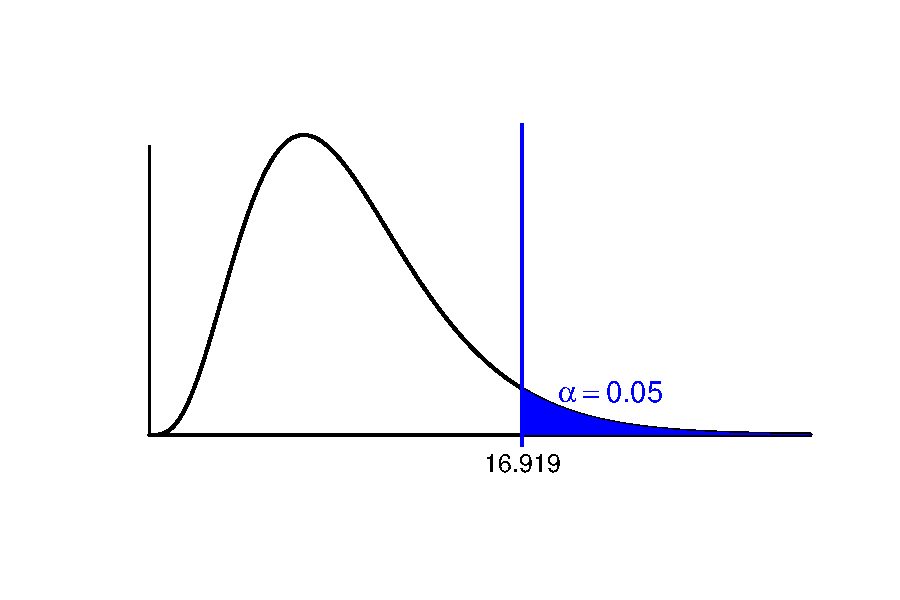
\includegraphics[width=0.70\textwidth]{section11/images/chisq_right_tail.pdf} 
\vspace{-3em} % ← reduce space between figure and caption
\captionsetup{skip=0pt}
\caption{Right-tailed chi-squared distribution with critical value at 16.919.}
\end{figure}

\textbf{Step 4. Conclusion.} \\
The $\chi^2$ statistic is not significant at the 0.05 level. We conclude that there is insufficient evidence to claim that $\sigma > 0.9$ year.
\end{example}
















